\section{解决一个实际用例：二元函数}

本教程假设我们有两个函数需要绘图：第一个是由一个巨大数据文件给出的
采样函数，第二个是数学表达式 $g(x,y)=\exp(-x^2-y^2)\cdot x$。

我们的第一个函数其实由两个数据文件构成：第一个文件包含
一些散乱数据，它们像是某个函数的离散化（“采样”），第二个
文件包含函数本身在网格上采样的数据。这里的需求是把\emph{两个}图画进
同一个坐标轴：一幅把函数画成平滑、着色的曲面，另一幅把散乱数据文件
放在曲面之上，因为它提供了计算机中如何表示该函数的
更多细节。

第二个以数学表达式给出的函数应当用等高线图
来可视化。等高线图期待若干固定值 $g_1, \dotsc,
g_k$ 作为输入（即等高值），并对每个 $g_j = g(x,y)$
画一条曲线（也就是说，如果你去徒步，路径高度始终不变）。


\subsection{从数据文件绘制曲面图}

我们的第一步是加载数据文件并绘制曲面。

显然，二元函数需要更复杂的输入格式：
它们通常在 $n \times m$ 个点的统一网格上采样，即
$x$ 方向 $n$~个点、$y$ 方向 $m$~个点，总共得到一个含
$n\cdot m$ 个值 $f_{ij} = f(x_i,y_i)$ 的矩阵。我们如何读取矩阵数据？如果
你拥有的不只是 $z$ 值又怎么办？一种标准做法是把矩阵
写成一张表，既可按行排列，也可按列排列
（两种都常见）。

这里，我们假设函数值被写进一张表，其中
$y$ 值逐行变化。下面是该数据文件的一段摘录
（文件太大，无法在此完整列出）：

    \lstinputlisting[
        columns=fixed,
        breaklines=false,
        firstline=1,
        tabsize=15,
        lastline=6,
    ]{plotdata/concat_VV_together.dat}%
        \vskip-0.9\baselineskip
            $\vdots$
        \vskip-0.4\baselineskip
    \lstinputlisting[
        columns=fixed,
        breaklines=false,
        firstline=34,
        tabsize=15,
        lastline=43,
    ]{plotdata/concat_VV_together.dat}%
        \vskip-0.9\baselineskip
            $\vdots$

注意，该数据文件（以及本手册中引用的所有其他文件）都随
\PGFPlots{} 一起发布；你可以在子文件夹
\texttt{doc/latex/pgfplots/plotdata} 中找到它们。

输入文件在名为 |x_0|、|x_1| 和 |f(x)| 的列中分别包含 $x_0$、$x_1$
和 $f(x_0,x_1)$。此外，它还包含一些与这里无关的元数据。

注意，每当 |x_0| 变化时，我们的输入文件中就出现\emph{空行}。
这是一种常见数据格式，它简化了“扫描线长度”的检测。
一条扫描线就是输入矩阵中的一行，例如由所有满足
$x_0 = 0$ 的点组成的那一行。有了这样的扫描线，\PGFPlots{} 就能
自动推断输入矩阵的尺寸。

为了把该文件绘制成曲面，我们像前面的示例那样使用
|\addplot table|。不过，我们必须使用 |\addplot3| 以表明
期待一个三维结果：\pgfplotsexpensiveexample
%
\begin{codeexample}[]
\begin{tikzpicture}
\begin{axis}
    \addplot3 [
        surf,
        mesh/ordering=y varies,
    ] table {concat_VV_together.dat};
\end{axis}
\end{tikzpicture}
\end{codeexample}
%
与前面几个教程的结果相比，这个示例看起来很眼熟：
一个 |tikzpicture| 环境，内含一个 |axis| 环境以及上面提到的
|\addplot3| 命令。选项列表包含 |surf|，它告诉 \PGFPlots{}
如何可视化输入数据。键 |mesh/ordering=y varies| 告诉
\PGFPlots{} 如何解码输入矩阵。这很重要；否则
\PGFPlots{} 会选择 |x varies|，而它与我们的文件不匹配。

注意，这里无需配置 |mesh/rows=|\meta{N} 或
|mesh/cols=|\meta{N}，因为这些参数会根据输入文件中
空行所标记的扫描线长度自动推断出来。

由于我们的 |\addplot3 table| 语句没有任何关于该绘制哪些列的提示，
\PGFPlots{} 只是把前三列两两相对
绘制出来。

|surf| 图的颜色由函数值选取（除非你
为 |point meta| 配置了其他值；这与散点图
示例类似）。对于二元函数，函数值就是
第三列。


\subsection{微调}

为强调颜色应如何映射到数值，我们给上一小节的
示例加上颜色条。此外，我们把视角
稍微旋转一下，并加上坐标轴标签。而且，我们希望得到平滑的
颜色映射。

最终得到
%
\pgfplotsexpensiveexample
\begin{codeexample}[]
\begin{tikzpicture}
\begin{axis}[
    view/h=40,
    colorbar horizontal,
    xlabel=$x$, ylabel=$y$,
]
    \addplot3 [
        surf,
        mesh/ordering=y varies,
        shader=interp,
    ] table {concat_VV_together.dat};
\end{axis}
\end{tikzpicture}
\end{codeexample}
%
这里，|view/h|（只）旋转视图的“水平”部分。它为
正交投影选择一个新的视角。正如你猜到的，还有
一个 |view/v| 键和一个 |view=|\marg{h}\marg{v} 变体。

键 |colorbar horizontal| 是一个样式，它激活 |colorbar| 并
配置其水平显示。标签像我们前面看到一维
函数可视化时那样，用 |xlabel| 和 |ylabel| 放置。颜色条使用当前的
|colormap|，并加上坐标轴描述，以展示数值如何映射到
颜色。

键 |shader=interp| 激活平滑的颜色插值。


\subsection{把散乱数据加到曲面之上}

如前所述，我们有第二个数据集，它刻画了
函数在某个计算机模拟中是如何表示的。我们想把
第二个数据集作为散点图加在函数
之上。

这个数据集本身与 Section~\ref{sec:tut3:usecaseA} 中
所用的完全相同，所以这里不再列出。
不过，我们必须以合适的方式把二维散点数据
纳入三维坐标轴。我们选择把它放在一个固定的 $z$
值上，如下所示：
%
\pgfplotsexpensiveexample
\begin{codeexample}[]
\begin{tikzpicture}
\begin{axis}[
    view/h=40,
    colorbar horizontal,
    xlabel=$x$, ylabel=$y$,
]
    \addplot3 [surf,mesh/ordering=y varies,
        shader=interp
    ] table {concat_VV_together.dat};

    \addplot3 [blue,mark=*,
        mark options={fill=blue!80!black},
        only marks,mark size=0.6pt,
    ] table [z expr=1.2]{concat_VV_together_grid.dat};
\end{axis}
\end{tikzpicture}
\end{codeexample}
%
现在，同一个坐标轴里有两条 |\addplot3 table| 语句。它们都没有
使用 |cycle list|，因为我们使用了显式选项列表。第一条是我们的
曲面图。注意，它在散点图之前绘制：\PGFPlots{}
无法处理相邻 |\addplot| 语句之间的深度信息。不过，
它能处理单条 |\addplot| 语句内部数据的 |z buffer|
信息。第二幅图是散点图：我们认出了
Section~\ref{sec:tut3:usecaseA} 中的 |only marks| 和
|mark size|。此外，我们还配置了
一些颜色和标记选项。

一个重要方面是 |\addplot3 table[z expr=1.2]|——它告诉 \PGFPlots{}
如何为输入文件选择 $z$ 值（否则，\PGFPlots{} 会使用
该文件的第三列）。这是把
二维数据插入三维坐标轴的便捷方式，前提是你拥有
\emph{表}数据。还有另一种方式，它同时适用于表
和数学表达式（或其他输入类型）。这另一种方式是安装一个
|z filter|，不过目前超出了本教程的范围。


\subsection{计算数学表达式的等高线图}

本节处理用例示例的第二部分：一个
以数学表达式给出的二元函数。

我们感兴趣的函数是 $x \exp(-x^2-y^2)$。我们像一维
函数教程中那样起步，即由数学表达式给出函数（比较
Section~\ref{sec:tut1:step3}）：使用一条 |\addplot| 语句，其后
跟一个花括号中的数学表达式。不过，我们像上一节那样使用 |\addplot3|：

\pgfplotsexpensiveexample
\begin{codeexample}[]
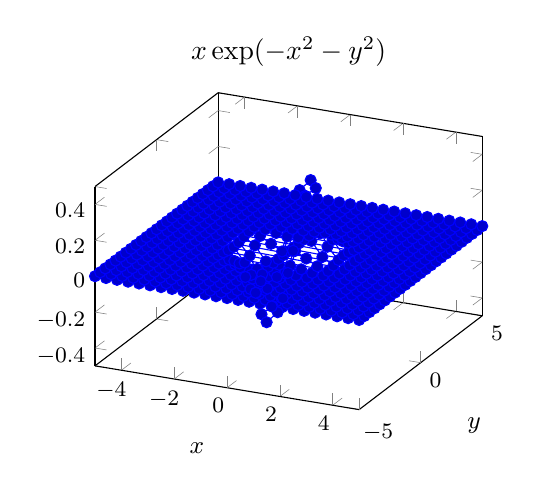
\begin{tikzpicture}
\begin{axis}[
    title={$x \exp(-x^2-y^2)$},
    xlabel=$x$, ylabel=$y$,
    small,
]
    \addplot3 {exp(-x^2-y^2)*x};
\end{axis}
\end{tikzpicture}
\end{codeexample}
%
我们的示例包含一个基本的坐标轴环境，带有前面几个教程中
已经见过的 |title|、|xlabel|、|ylabel| 和 |small| 键。
|\addplot3| 没有选项，后面紧接着就是数学表达式。
没有选项这一点告诉 \PGFPlots{} 使用它的 |cycle list|。这
进而配置了带 |blue| 颜色的 |mark=*|——以及一幅线图。
线图与 |\addplot3| 组合用处有限；它只是把所有
传入的点连接起来。由于点是以矩阵方式采样的（逐行）。我们下一步
将定义一个合适的绘图处理器。

不过注意，我们的数学表达式依赖 |x| 和 |y|。在 \PGFPlots{} 的默认
配置中，这两个变量就是采样变量：
二者都在感兴趣的 |domain| 内用正确数量的
|samples| 采样。|\addplot3| 语句负责按正确的顺序计算 $N\cdot M$ 个点，
其中 $N$ 是 $x$ 的 |samples| 数，$M$ 是
|samples y|，即 $y$ 的采样数。

我们可以看到采样 |domain| 太大。换成更小的
|domain| 可以聚焦到函数的有趣部分：

\pgfplotsexpensiveexample
\begin{codeexample}[]
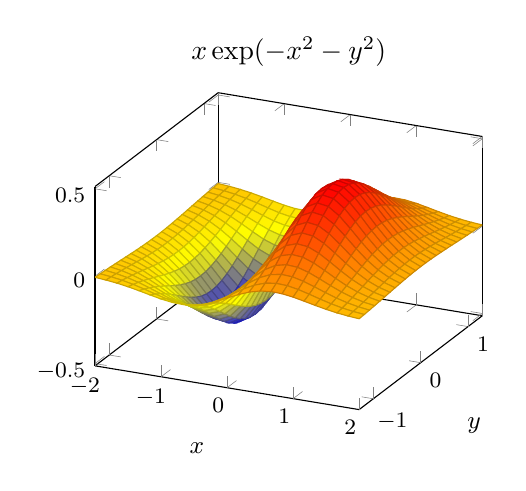
\begin{tikzpicture}
\begin{axis}[
    title={$x \exp(-x^2-y^2)$},
    xlabel=$x$, ylabel=$y$,
    small,
]
    \addplot3 [
        surf,
        domain=-2:2,
        domain y=-1.3:1.3,
    ] {exp(-x^2-y^2)*x};
\end{axis}
\end{tikzpicture}
\end{codeexample}
%
这里，我们在 |\addplot3| 之后加了一个选项列表。由于我们
提供选项列表时没有前导加号 `|+|'，\PGFPlots{}
完全不考虑它的 |cycle list|（并关闭 |mark| 和默认
颜色设置）。我们加上 |domain| 和 |domain y|，以便以合适的方式
限制采样域。如果省略 |domain y|，$y$ 域
会使用与 $x$ |domain| 相同的值。

正如你可能猜到的，|surf| 键的主要用途是与上一节教程建立
联系：它是二元函数最自然的
可视化方式之一。与上一节一样，
颜色由函数值 $z=f(x,y)$ 推出（更确切地说，
依赖默认配置 |point meta=f(x)|）。

下一步是把 `|surf|' 换成 `|contour lua|'，从而改用等高线图：

\pgfplotsexpensiveexample
\begin{codeexample}[]
\begin{tikzpicture}
\begin{axis}[
    title={$x \exp(-x^2-y^2)$},
    xlabel=$x$, ylabel=$y$,
    small,
]
    \addplot3 [
        contour lua,
        domain=-2:2,
        domain y=-1.3:1.3,
    ] {exp(-x^2-y^2)*x};
\end{axis}
\end{tikzpicture}
\end{codeexample}
%
现在，我们得到了一幅等高线图——虽然它还不完全是我们想要的。
首先，等高线太少，很难看清任何东西
（尤其是因为 |line width| 太小）。此外，|view|
方向也很陌生。

我们加上 |view| 选项，参数取“俯视”，并用
|contour/number| 键配置等高线数量，用 |thick|
样式配置 |line width|：

\pgfplotsexpensiveexample
\begin{codeexample}[]
\begin{tikzpicture}
\begin{axis}[
    title={$x \exp(-x^2-y^2)$},
    enlarge x limits,
    view={0}{90},
    xlabel=$x$, ylabel=$y$,
    small,
	colorbar,
]
    \addplot3[
        domain=-2:2,
        domain y=-1.3:1.3,
        contour lua={number=14,labels=false},
        thick,
    ] {exp(-x^2-y^2)*x};
\end{axis}
\end{tikzpicture}
\end{codeexample}

这正是我们想达到的效果。注意，|contour lua| 接受
那些键前缀为 |contour/| 的选项。在此上下文中，该前缀是
可选的。

注意，|contour lua| 在一个方面与 \PGFPlots{} 几乎所有其他绘图处理器
都不同：它要求你调用

|lualatex |\meta{texfilename}

\noindent 而不是

|pdflatex |\meta{texfilename} .

\noindent
计算等高线的非线性算法目前在 plain \TeX{} 中尚不可用，
这一点由名字 `|contour lua|' 强调。


如果你因某种原因无法使用 |lualatex|，可以把 |contour lua| 换成 |contour gnuplot|，前提是你的系统上安装了外部程序 |gnuplot|（更多细节参见 |contour gnuplot| 的参考）。

\subsection{小结}

我们勾勒了如何加载一张包含二元采样函数的数据表，并学习了
如何把这样的数据可视化为 |surf|ace 图。我们学习了如何旋转
|view|，如何改变 |surf|ace 图的颜色 |shader|，如何启用
|colorbar|，以及如何把 |scatter| 图加到曲面图之上。此外，我们以
第一幅等高线图为例，看到了如何借助 \PGFPlots{} 的内置
方法对二元函数采样。

需要强调的是，\PGFPlots{} 生成这类图不需要任何外部
工具：任何装有较新版本 \PGFPlots{} 的计算机都能重新生成这些图。

关于三维坐标轴，可讲的还有很多，尤其是
|mesh/ordering|、参数图，也许还有三维线图或
其他图类型。此外，|z buffer|ing 存在一些
局限，即 \PGFPlots{} 如何决定图的哪些部分
位于其他部分之前。这些内容可在 Section~\ref{sec:3d} 及其
小节中阅读。

你可能还对改变三维坐标轴外观的样式感兴趣，
比较 Section~\ref{sec:3d:axis:config}。
